\section{Mocniny, mocninná funkce}

\begin{definition}
    Nechť $n\in \mathbb N.$ Pak funkci $f: y=x^n$ nazýváme \textbf{mocninnou funkcí}
    s~přirozeným exponentem.
\end{definition}

\begin{definition}
    Nechť $n\in \mathbb N.$ Pak funkci $f: y=x^{-n}=\frac{1}{x^n}$ nazýváme
    \textbf{mocninnou funkcí} s~celým záporným exponentem.
\end{definition}

\begin{definition}
    Nechť $\frac{p}{q}\in \mathbb Q, x \in \mathbb R^+.$ Pak funkci $f: y=
    x^{\frac{p}{q}}=\sqrt[q]{x^p}$ nazýváme \textbf{mocninnou funkcí}
    s racionálním exponentem.
\end{definition}


\begin{figure}[ht!]
  \centering
  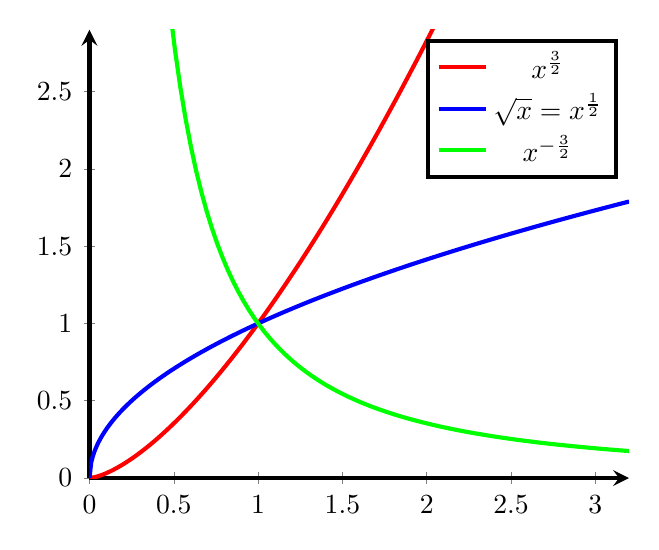
\begin{tikzpicture}
    \begin{axis}[
        axis lines = left,
        ymin=0,
        ymax=2.9,
        xmin=0,
        xmax=3.2,
        line width=1.5pt,
    ]
    %Below the red parabola is defined
    \addplot [
        domain=0:3.2,
        samples=100,
        color=red,
    ]
    {x^(3/2)};
    \addlegendentry{\(x^\frac{3}{2}\)}

    \addplot [
        domain=0:3.2,
        samples=300,
        color=blue,
        ]
        {sqrt(x)};
    \addlegendentry{\(\sqrt{x}=x^\frac{1}{2}\)}

    \addplot [
        domain=0.1:3.2,
        samples=100,
        color=green,
        ]
        {x^(-3/2)};
    \addlegendentry{\(x^{-\frac{3}{2}}\)}

    \end{axis}
    \end{tikzpicture}
  \caption{Grafy různých mocninných funkcí}
\end{figure}

\begin{veta}[Pravidla pro počítání s mocninami]
    $\forall a \in \mathbb R, m,n \in \mathbb N:$
    \begin{enumerate}[$i.$]
        \item $a^m\cdot a^n=a^{m+n};$
       	\item $(ab)^n = a^n\cdot b^n;$
       	\item $a^m : a^n = a^{m-n}, a \ne 0;$
       	\item $(a : b)^n = a^n : b^n, b \ne 0;$
       	\item $\left ( a^m \right )^n = a^{mn}.$
    \end{enumerate}
\end{veta}

\begin{proof}
    Zřejmé.
\end{proof}

\begin{veta}
  Vlastnosti mocninných funkcí $y= x^n$, kde $n$ je přirozené číslo:
  \begin{enumerate}[1.]
    \item Pokud $n$ je liché.
    \begin{enumerate}[$i.$]
      \item $D(f)= \mathbb R$, $H(f)= \mathbb R$.
      \item Je lichá.
      \item Není omezená shora ani zdola.
      \item Je rostoucí v celém svém definičním oboru.
      \item Nemá maximum, ani minimum.
    \end{enumerate}
    \item Pokud $n$ je sudé.
    \begin{enumerate}[$i.$]
      \item $D(f)= \mathbb R$, $H(f)= \langle 0,+\infty )$.
      \item Je sudá.
      \item Není omezená shora, je zdola omezená.
      \item Je rostoucí v intervalu $\langle 0,+\infty )$, je klesající v intervalu $( -\infty,0 \rangle $.
      \item Nemá maximum, má minimum v bodě $0$.
    \end{enumerate}
  \end{enumerate}
\end{veta}

\begin{veta}
  Vlastnosti mocninných funkcí $y= x^{-n}$, kde $n$ je přirozené číslo:
  \begin{enumerate}[1.]
    \item Pokud $n$ je liché.
    \begin{enumerate}[$i.$]
      \item $D(f)= \mathbb R \smallsetminus \{ 0\}$, $H(f)= \mathbb R \smallsetminus \{ 0 \}$.
      \item Je lichá.
      \item Není omezená shora ani zdola.
      \item Je klesající v $( -\infty,0)$ a v $( 0,+\infty )$.
      \item Nemá maximum, ani minimum.
    \end{enumerate}
    \item Pokud $n$ je sudé.
    \begin{enumerate}[$i.$]
      \item $D(f)= \mathbb R \smallsetminus \{ 0\}$, $H(f)= ( 0,+\infty )$.
      \item Je sudá.
      \item Není omezená shora, je zdola omezená.
      \item Je rostoucí v intervalu $( -\infty,0 ) $, je klesající v intervalu $( 0,+\infty )$.
      \item Nemá maximum ani minimum.
    \end{enumerate}
  \end{enumerate}
\end{veta}

\begin{definition}
    Nechť $n\in \mathbb N, n\geq 2, x \geq 0.$ Pak inverzní funkci k funkci
    $f:y=x^n$ nazýváme \textbf{$n$-tou odmocninou} a značíme $f^{-1}: y=\sqrt[n]{x}.$
\end{definition}

\begin{veta}[Pravidla pro počítání s odmocninami]
    $\forall a,b \in \mathbb R, a,b \geq 0, m,n \in \mathbb N:$
    \begin{enumerate}[$i.$]
        \item $\sqrt[m]{a}\cdot \sqrt[m]{b}=\sqrt[m]{ab};$
       	\item $\sqrt[m]{\sqrt[n]{a} } = \sqrt[mn]{a};$
       	\item $\sqrt[m]{a} : \sqrt[m]{b} = \sqrt[m]{a:b};$
       	\item $\left ( \sqrt[m]{a}  \right )^n = \sqrt[m]{a^n};$
       	\item $\forall k \in \mathbb N: \sqrt[m]{a}=\sqrt[km]{a^k}.$
    \end{enumerate}
\end{veta}

\begin{proof}
    Zřejmé.
\end{proof}

\begin{veta}
    Vlastnosti odmocninných funkcí $y= \sqrt[n]{x}$, kde $n$ je přirozené číslo větší
    než jedna:
    \begin{enumerate}[$i.$]
        \item Není ani lichá, ani sudá.
       	\item Je rostoucí.
        \item Je zdola omezená.
        \item Má ostré minimum v bodě $(0,0).$
        \item Není periodická.
    \end{enumerate}
\end{veta}
